%% $Id: louveaux-epfl06.tex,v 1.5 2006/07/10 13:46:20 louveaux Exp $
%%\documentclass[9pt,trans]{beamer}
\documentclass[9pt]{beamer}
\usepackage{beamerfoils}%% FoilTeX emulation
\usepackage{epsfig}
\usepackage{eurosym}
\mode<presentation>
{
  \usetheme{Boadilla}
  % oder ...

  \setbeamercovered{transparent}
  % oder auch nicht
}
\usepackage[french]{babel}
\usepackage[latin1]{inputenc}
%%\usepackage{times}
%%\usepackage[T1]{fontenc}
%\usepackage{booktabs}

%%\includeonlyframes{current}

\title{Discrete Optimization}

\author{Quentin
Louveaux}
\institute{ULg - Institut Montefiore}
\date{2016}

% Falls eine Logodatei namens "university-logo-filename.xxx" vorhanden
% ist, wobei xxx ein von latex bzw. pdflatex lesbares Graphikformat
% ist, so kann man wie folgt ein Logo einf|gen:

% \pgfdeclareimage[height=0.5cm]{university-logo}{university-logo-filename}
% \logo{\pgfuseimage{university-logo}}

% Folgendes sollte gelvscht werden, wenn man nicht am Anfang jedes
% Unterabschnitts die Gliederung nochmal sehen mvchte.
%% \AtBeginSection[]
%% {
%%   \begin{frame}<beamer>
%%     \frametitle{Gliederung}
%%     \tableofcontents[currentsection,currentsubsection]
%%   \end{frame}
%% }

% Falls Aufzdhlungen immer schrittweise gezeigt werden sollen, kann
% folgendes Kommando benutzt werden:

\beamerdefaultoverlayspecification{<+->}

%%%%%%
\definecolor{rot}{rgb}{1,0,0}
\definecolor{gruen}{rgb}{0,1,0}
\definecolor{blau}{rgb}{0,0,1}

%%% number sets
\newcommand{\Z}       {\mathbb{Z} }
\newcommand{\R}       {\mathbb{R} }
\newcommand{\Q}       {\mathbb{Q} }
\newcommand{\N}       {\mathbb{N} }
\newcommand{\spa}     {\text{span}}
\newcommand{\lin}     {\text{span}}
\newcommand{\inter}   {\text{int} }


%%% mathematical stuff
\newcommand{\sosR}    {\sum^2}
\newcommand*{\transpose}[1]  { {#1}^T }
\newcommand*{\rounddown}[1]  {\left\floor #1 \right\rfloor}
\newcommand*{\roundup}[1]    {\left\lceil  #1 \right\rceil}
\newcommand*{\ipart}[1]      {\rounddown{#1}}
\newcommand*{\fpart}[1]      {\mathfrak{f}\left(#1\right)}


\newcommand*{\iepoly}[2]  {z_{#1}\left(#2\right)}
\newcommand*{\redmon}[3]  {r_{#1}^{#2}\left( #3 \right)}
\newcommand*{\redset}[1]  {#1^{\emph{red}}}

\newcommand*{\Gpoly}[1] {P_{[#1]}}

\newcommand*{\nonc}[1]{\overline{#1}}
\newcommand*{\const}[1]{#1_0}

\newcommand{\define}{\stackrel{\rm def.}{\Leftrightarrow}}
\newcommand{\qform}[3]{\frac{1}{2} x^{\top}#1x + #2^{\top}x + #3}
\def\xzero{x^{0}}
\newcommand{\gxh}[2]{{g_{#1}(#2)}}

\def\pcone_k{{\mathcal C}_{k}(f)}
\def\orthant_j{{\mathcal O}_{j}}

\def\BDB{BDB^{\top}}
\def\LDL{LDL^{\top}}
\def\bA{A}
\def\bb{b}
\def\bc{c}
\def\bh{h}
\def\bp{p}
\def\bx{x}
\def\by{y}
\def\bu{u}
\def\bv{v}
\def\bd{d}
\def\T{^{T}}
\def\D{}
\def\mb{{\bf}}
\def\sep{}
\def\bo{0}
\def\bw{w}
\def\ba{a}
\def\bg{g}
\def\bH{H}
\def\be{e}

\let\ve=\relax
\newcommand\vealpha{{\alpha}}
\newcommand{\st}{\mathrm{s.t.}}
\DeclareMathOperator\conv{conv}
\DeclareMathOperator\cone{cone}
\newcommand{\B}{\{0,1\}}

\newcommand*{\person}[1] {\textsc{#1}}

\newtheorem{algorithm}{Algorithmus}

\makeatletter
\newenvironment{rmat}{\left(\null\,\vcenter\bgroup
  \Let@\restore@math@cr\default@tag
  \baselineskip6\ex@ \lineskip1.5\ex@ \lineskiplimit\lineskip
  \ialign\bgroup\hfil$\m@th\scriptstyle##$&&\thickspace
  \hfil$\m@th\scriptstyle##$\crcr
}{%
  \crcr\egroup\egroup\,\right)%
}
\makeatother

%%%%%%%%%%%%%%%%%%%%%%%%%%%%%%%%%%%%%%%%%%%%%%%%%%%%%%%%%%%%%%%%%%%%%%%%%%%%%%%%
%\begin{frame}
  %\titlepage
%\end{frame}

%% \begin{frame}
%%   \frametitle{Gliederung}
%%   \tableofcontents
%%   % Die Option [pausesections] kvnnte n|tzlich sein.
%% \end{frame}


%%%%%%%%%%%%%%%%%%%%%%%%%%%%%%%%%%%%%%%%%%%%%%%%%%%%%%%%%%%%%%%%%%

\definecolor{orange}{rgb}{0.8,0.3,0.0}
\definecolor{darkgreen}{rgb}{0.0,0.5,0.0}
\definecolor{gold}{rgb}{1.0,0.8,0.0}
\definecolor{brown}{rgb}{0.6,0.2,0.2}
\definecolor{blue4}{rgb}{0,0,144}
\definecolor{white}{rgb}{255,255,255}
\definecolor{blueexample}{rgb}{0.2,0.2,0.7}
\begin{document}
\begin{frame}
  \titlepage
\end{frame}
\begin{frame}
\frametitle{Comparing two formulations}
To compare \alert{two formulations} $P^1$ and $P^2$ with
the same \alert{integer feasible points}, we consider
their respective \alert{linear relaxations} $P^1_{LP},P^2_{LP}$.
\bigskip

\uncover<2->{\begin{block}{Comparing two formulations}\noindent $P^1$ is \alert{better} than $P^2$ 
if $$P^1_{LP} \subset P^2_{LP}$$\end{block}}

\uncover<3->{\begin{block}{Ideal formulation}
If $\mathcal F=\{x_1,\ldots,x_k\}$ is the set of
\alert{feasible solutions}, an \alert{ideal formulation} is
$$\conv(\mathcal F)$$\end{block}}

\end{frame}
\begin{frame}
\frametitle{Comparing two formulations: the facility location problem}
In the uncapacitated facility location problem (UFL), we are given a set of potential facilities (with a fixed cost $f_i$ when open) to open to serve a list of clients (with cost $c_{ij}$).\\
What is the set of facilities to open, and which clients should they serve in order to minimize the cost?
\begin{block}{Variables}
$y_i = 1$ if facility $i$ is open (0 otherwise)\\
$x_{ij}=1$ if facility $i$ serves client $j$ (0 otherwise)
\end{block}
\begin{minipage}{.49\linewidth}
\begin{center}
\textbf{Formulation 1}
\end{center}
\begin{align*}
\min \; & \sum_i f_i y_i + \sum_{i,j} c_{ij} x_{ij}\\
\text{subject to } & \sum_i x_{ij} = 1 \quad \text{for all } j\\
& x_{ij} \leq y_i\\
& x_{ij}\in \{0,1\}, y_i\in \{0,1\}.
\end{align*}
\end{minipage}
\begin{minipage}{.49\linewidth}
\begin{center}
\textbf{Aggregated formulation}
\end{center}
\begin{align*}
\min \; & \sum_i f_i y_i + \sum_{i,j} c_{ij} x_{ij}\\
\text{subject to } & \sum_i x_{ij} = 1 \quad \text{for all } j\\
& \sum_{j=1}^n x_{ij} \leq n y_i\\
& x_{ij}\in \{0,1\}, y_i\in \{0,1\}.
\end{align*}
\end{minipage}
\end{frame}
\begin{frame}
\frametitle{Comparing two formulations for graph problems}
\begin{block}{The minimum spanning tree}
Let $G=(V,E)$ be an undirected graph. Every edge has a \alert{cost $c_e$}.
We look for the tree with the \alert{minimum total cost}.
\begin{overlayarea}{\linewidth}{4cm}
\begin{center}
\includegraphics<1>[width=.3\linewidth]{mst1.pdf}
\includegraphics<2->[width=.3\linewidth]{mst2.pdf}
\end{center}
\end{overlayarea}
\end{block}
\uncover<3->{Constraints to encode:}
\begin{itemize}
\item<4-> A tree should have \alert{$n-1$ edges} where $n$ is the number of nodes
\item<5-> A tree \alert{cannot have a cycle} or equivalently\\
A tree must be \alert{connected}
\end{itemize}
\end{frame}
\begin{frame}
\frametitle{Subtour elimination formulation}
\begin{block}{Integer formulation}
\begin{align*}
P^I_{sub} = \{ x_e \in \{0,1\} \mid & \sum_{e\in E} x_e=n-1\\
& \sum_{e\in E(S)} x_e \leq |S|-1, \quad S\subset V, S\neq \emptyset, V\;\}
\end{align*}
\end{block}
\begin{block}{Linear programming relaxation}
\begin{align*}
P_{sub} = \{ x_e \in \alert{[}0,1\alert{]} \mid & \sum_{e\in E} x_e=n-1\\
& \sum_{e\in E(S)} x_e \leq |S|-1, \quad S\subset V, S\neq \emptyset, V\;\}
\end{align*}
\end{block}
\end{frame}
\begin{frame}
\frametitle{Cutset  formulation}
\begin{block}{Integer formulation}
\begin{align*}
P^I_{cut} = \{ x_e \in \{0,1\} \mid & \sum_{e\in E} x_e=n-1\\
& \sum_{e\in \delta(S)} x_e \geq 1, \quad S\subset V, S\neq \emptyset, V\;\}
\end{align*}
\end{block}
\begin{block}{Linear programming relaxation}
\begin{align*}
P_{cut} = \{ x_e \in \alert{[}0,1\alert{]} \mid & \sum_{e\in E} x_e=n-1\\
& \sum_{e\in \delta(S)} x_e \geq 1, \quad S\subset V, S\neq \emptyset, V\;\}
\end{align*}
\end{block}
\end{frame}
\begin{frame}
\frametitle{Comparing the two formulations}
\begin{block}{Theorem}
\begin{itemize}
\item $P_{sub}\subset P_{cut}$ and the inclusion is sometimes strict
\item $P_{cut} $ can have fractional extreme points
\end{itemize}
\end{block}
\end{frame}
\begin{frame}
\frametitle{The traveling salesman problem}
\begin{block}{Subtour elimination formulation}
\begin{align*}
P^I_{tspsub} = \{ x_e \in \{0,1\} \mid & \sum_{e\in \delta(\{i\})} x_e=2\quad \text{for all }i\in V\\
& \sum_{e\in E(S)} x_e \leq |S|-1, \quad S\subset V, S\neq \emptyset, V\;\}
\end{align*}
\end{block}
\begin{block}{Cutset formulation}
\begin{align*}
P^I_{tspcut} = \{ x_e \in \{0,1\} \mid & \sum_{e\in \delta(\{i\})} x_e=2 \quad \text{for all } i\in V\\
& \sum_{e\in \delta(S)} x_e \geq 2, \quad S\subset V, S\neq \emptyset, V\;\}
\end{align*}
\end{block}
\begin{block}{Theorem}
If $P_{tspsub} $ and $P_{tspcut}$ are the respective linear relaxations,
$$P_{tspsub}=P_{tspcut}$$
\end{block}
\end{frame}
\begin{frame}
\frametitle{The matching problem}
Consider a set of $N$ pilots that must be matched by teams of two.\\
Each pilot has certain skills (languages that he speaks, operations that he is able to perform,
\ldots)\\
\uncover<2->{For each \alert{pair of pilots}, we define a \alert{reward} $c_{ij}$
that corresponds to the fact that these two pilots are matched together.\bigskip}

\uncover<3->{\noindent What is the best way to divide the $n$ pilots
into \alert{$\frac{N}{2}$ teams of 2 pilots} in order to maximize the reward.}
\begin{center}
\includegraphics<1-2>[width=.4\linewidth]{matching.pdf}
\includegraphics<3>[width=.4\linewidth]{matching_red.pdf}
\end{center}
\end{frame}
\begin{frame}
\frametitle{The matching problem}
\begin{block}{Simple formulation}
\begin{align*} 
\text{minimize} \;&\sum_{e\in E} c_ex_e\\
\text{subject to}\;& \sum_{e\in \delta(\{i\})} x_e = 1\\
& x_e\in \{0,1\}
\end{align*}
The linear relaxation is \alert{not the convex hull} of all
feasible solutions.
\end{block}
\begin{block}{Enhanced formulation}
\begin{align*} 
\text{minimize} \;&\sum_{e\in E} c_ex_e\\
\text{subject to}\;& \sum_{e\in \delta(\{i\})} x_e = 1\\
&\sum_{e\in \delta(S)}x_e\geq 1\qquad S\neq V, |S| \ \text{odd}\\
& x_e\in \{0,1\}
\end{align*}
\end{block}
\end{frame}
\begin{frame}
\frametitle{The Steiner tree problem}
Given a graph and some \alert{terminal nodes},
find the shortest tree that connects all terminal nodes.\\
Very similar to the minimum spanning tree but this version is \alert{NP-hard}!
\begin{center}
\includegraphics<1>[width=.5\linewidth]{steiner_instance.pdf}
\includegraphics<2>[width=.5\linewidth]{steiner_sol.pdf}
\end{center}
\end{frame}
\begin{frame}
\frametitle{Steiner tree real-world instance}
\begin{center}
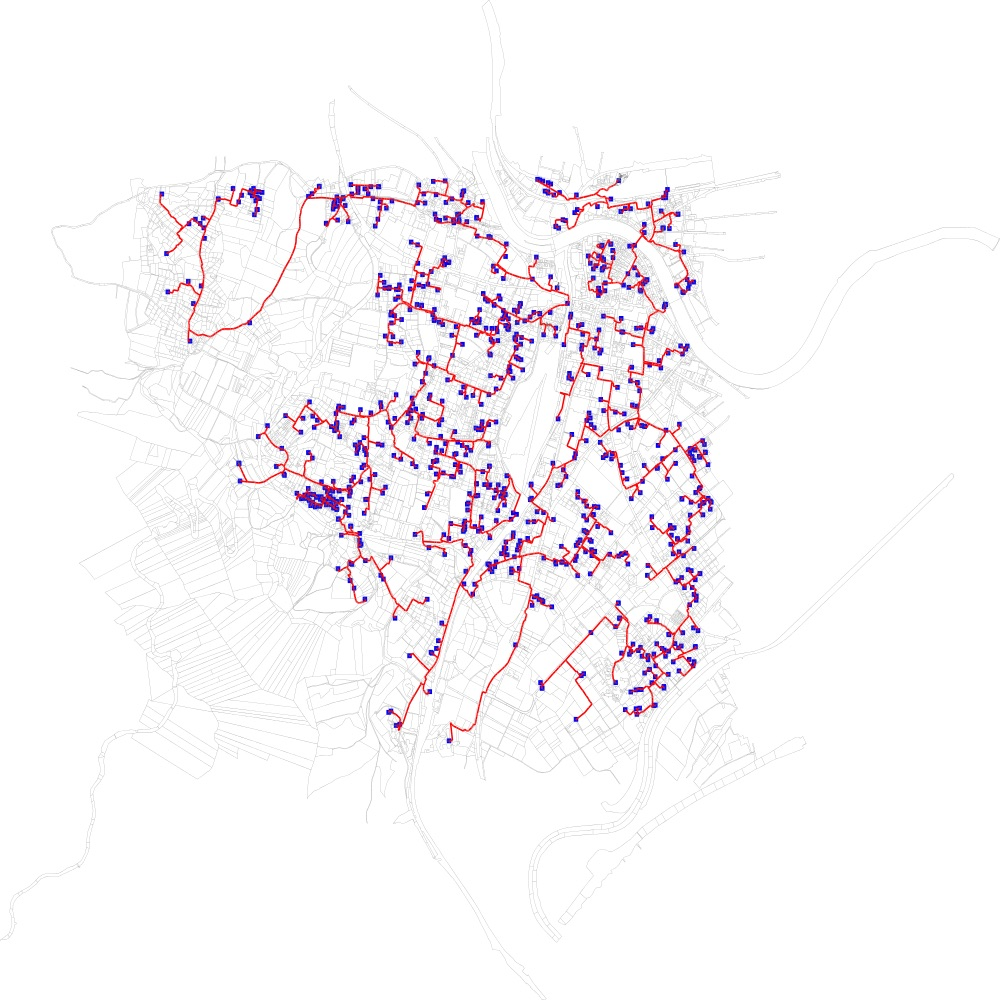
\includegraphics[width=\linewidth]{U-G107.jpg}
\end{center}
\end{frame}
\begin{frame}
\frametitle{3 formulations of the Steiner tree problem}
\begin{block}{Simple formulation}
\begin{align*} 
\text{minimize} \;&\sum_{e\in E} c_ex_e\\
\text{subject to}\;& \sum_{e\in \delta(S)} x_e \geq 1 \qquad S\subset V,\ S\cap T \neq \emptyset,T\\
& x_e\in \{0,1\}
\end{align*}
\end{block}
\begin{block}{Enhanced formulation}
\begin{itemize}
\item<1-> $V_i\cap T\neq \emptyset, i=1,\ldots, p$
\item<1-> $V_i\cap V_j=\emptyset, i\neq j$
\item<1-> $V_1 \cup \cdots \cup V_p = V$
\end{itemize}
\begin{align*} 
\text{minimize} \;&\sum_{e\in E} c_ex_e\\
\text{subject to}\;& \sum_{e\in \delta(V_1,\ldots,V_p)} x_e \geq p-1 \\
& x_e\in \{0,1\}
\end{align*}
\end{block}
\end{frame}
\begin{frame}
\frametitle{Directed formulation}
\begin{align*}
\text{minimize}\; & \sum_{(i,j)\in A} c_{ij} y_{ij}\\
\text{subject to}\; & \sum_{(i,j): i\in S, j\in V\setminus S} y_{ij} \geq 1, \quad S\subset V, 1\in S, S\cap T\neq T\\
& y_{ij}+y_{ji}\leq 1\\
& y_{ij}\in \{0,1\}
\end{align*}
\begin{block}{Comparing the formulations}
$$Z_{Steiner} \leq Z_{partition} \leq ZD_{steiner}$$
where Z correspond to \alert{linear relaxations}.
\end{block}
\end{frame}
\end{document}
